% New stuff
% + Gazebo (add it to intro, but let Rich discuss it)
% + RETF using Player as the basis for a forthcoming standard; mention the
%     upcoming special session / meeting at IROS
% + NSF project (Beyond LEGOs...; get the exact details from Douglas's
%     email) to develop undergrad robotics curricula using Player, with Stage 
%     as their standard simulator
% + Webots (mention it, in the context of industrial/community interest)
% + Two new releases made since last meeting: 1.3.2 & 1.4rc1.
% + New hardware support (crib from Release Notes for list).
% + Mention DGPS support in garminnmea driver.
% - Tell the story of John's writing the RMP driver, so as to stress the 
%     power of the Open Source model and an inclusive developer policy.
% - Renewed focus on implementing higher-level algorithms as drivers (crib 
%     from Release Notes for list).
% + Talk about AMCL and the sensor modalities that it supports.  Maybe get
%     an anectdote from BBN guys on using it with AmigoBots' sonar?
% + Talk about VFH+ driver and show videos of autonomous RMP
%     wall-following.
% + Added logfile support.
% + Resource discovery / name service: Reed's libservicediscovery support
%     and Player's more primitive name lookup.
% + New mapping utility.

\documentclass[30pt,landscape,magscalefonts]{foils}
\usepackage{floatflt}
\usepackage{tabularx}
\usepackage[pdftex]{graphicx}
\graphicspath{{./graphics/}}
\usepackage[pdftex]{color}
\usepackage[pdftex]{geometry}
\geometry{headsep=2.0em,hscale=0.80}
\usepackage{hyperref}
\hypersetup{
  pdftitle={SDR September 2003 Report on Player},
  pdfauthor={Brian P. Gerkey, USC Robotics Research Lab},
  pdfpagemode={FullScreen},
  pdfborder={0 0 0}
}

% define some nice colors
\definecolor{myred}{rgb}{0.6,0,0}
\definecolor{myblue}{rgb}{0,0.2,0.4}
\color{myblue}

% don't want any paragraph indentation
\setlength{\parindent}{0cm}

% wrapper for foilhead that sets the text color
\newcommand{\foilheadc}[1]{\foilhead{\Large \textcolor{myred}{#1}}\vspace*{-2em}}
% wrapper for itemize that shortens the inter-item separation
\newenvironment{xitemize}{\begin{itemize} \itemsep 1pt}{\end{itemize}}
% wrapper for enumerate that shortens the inter-item separation
\newenvironment{xenumerate}{\begin{enumerate} \itemsep 1pt}{\end{enumerate}}

\def\movieroot{file:///mnt/win/users/gerkey/videos}

\title{\textcolor{myred}
{\large \vspace*{-2.0em}\\The Player/Stage Project: Recent Advances in Robot Control and
Simulation\vspace*{0.5em}}}
\author{\small Brian P. Gerkey\hspace{1.5em} Richard T. Vaughan\hspace{1.5em}
Andrew Howard\vspace*{1em}\\

\includegraphics[height=20mm]{cres-logo.jpg}

\includegraphics[height=20mm]{usclogo.jpg}\hspace*{2em}

\includegraphics[height=20mm]{hrl_logo.jpg} \vspace*{0.5em}\\
{\tt http://playerstage.sourceforge.net}}
\date{}

\newcommand{\distfont}{\fontfamily{phv}\fontseries{b}\fontsize{8pt}{8pt}\selectfont}

% headers, etc.
\leftheader{
\includegraphics[height=15mm]{cres-logo.jpg}}
\rightheader{
\includegraphics[height=15mm]{usclogo.jpg}}
\MyLogo{\parbox{0.5\textwidth}{\distfont
Distribution authorized to U.S. Government Agencies and their contractors
for administrative or operational use on 9/22/03.  Other requests for
this document shall be referred to DARPA/IPTO.}}
%\MyLogo{}
\def\totalpages{\pageref{lastpage}}
\rightfooter{\textcolor{myblue}{\quad\textsf{\thepage/\totalpages}}}

\begin{document}

% the title slide
\maketitle

% get the page numbering right
\pagebreak\setcounter{page}{2}

%\MyLogo{\textcolor{myblue}{SDR PI Meeting, September 2003}}

\foilheadc{Project overview}
The Player/Stage project is a collaborative development effort aimed at
producing high-quality Open Source tools for robotics researchers.
\vfill
The project primarily maintains three pieces of software:
{\small
\begin{itemize}
\item {\bf Player}: networked robot device server
\item {\bf Stage}: scalable 2-D multiple robot simulator
\item {\bf Gazebo}: high-fidelity 3-D multiple robot simulator
\end{itemize}
}

\foilheadc{Usage}
\begin{center}
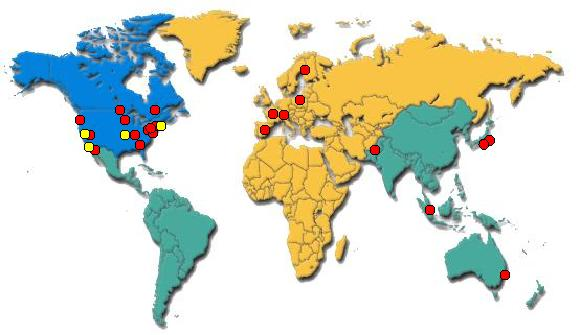
\includegraphics[height=120mm]{usage-map.jpg}
\end{center}

\foilheadc{Usage (cont'd)}
\begin{center}
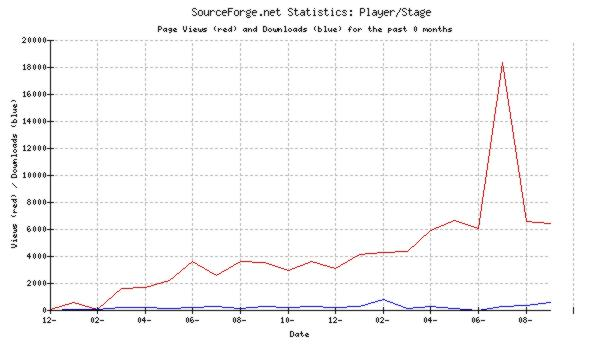
\includegraphics[height=130mm]{stats_graph.jpg}
\end{center}

\foilheadc{Misinterpretation by the press?}
\begin{center}
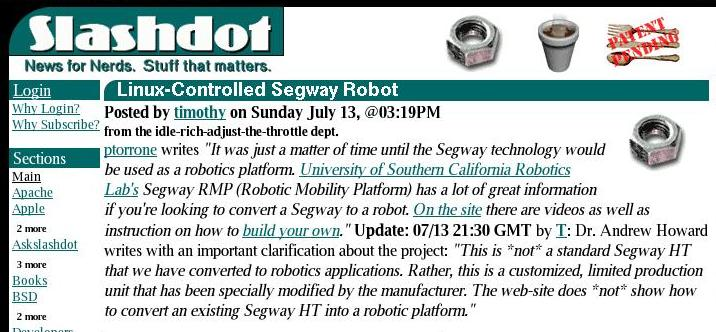
\includegraphics[width=1.0\textwidth]{slashdot_headline.jpg}
\end{center}

\foilheadc{Helping to explain things...}
\begin{center}
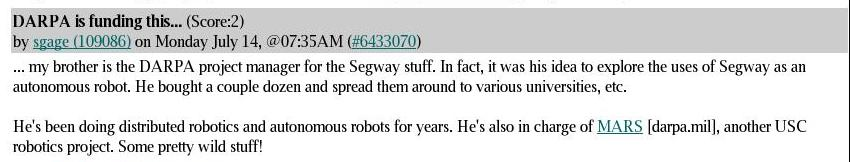
\includegraphics[width=1.1\textwidth]{slashdot_sgage_comment.jpg}
\end{center}

\foilheadc{Community interest}
{\small
\begin{xitemize}
\item RETF using the Player protocol as the basis for forthcoming standard
in robot device control (meeting next month at IROS).
\item NSF-funded project (``Beyond LEGOs: Building the next generation
robotics laboratory'') using Player \& Stage; to be deployed in a dozen
universities this fall.
\item Player interface to the Webots simulator (from Cyberbotics, Inc.) under
development.
\item Stage used as testbed for NASA/JPL's MDS.
\end{xitemize}
}

\foilheadc{Since last time\ldots}
\vspace*{-1em}
\begin{xitemize}
\item Two new releases: 1.3.2 \& 1.4rc1.
\item New hardware support (highlights):
{\small
\begin{xitemize}
\item Segway RMP {\tiny (John Sweeney @ UMass, Amherst)}
\item Non-Mobility control of RWI robots 
{\tiny (Matt Brewer @ UMass, Amherst)}
\item CMUCam {\tiny (James McKenna @ SAIC)}
\item NMEA-compliant (e.g., handheld) GPS units
\end{xitemize}
}
\item New high-level algorithms: 
{\small
\begin{xitemize}
\item AMCL  {\tiny (Andrew Howard @ USC, based on [Fox 2001])}
\item VFH+  {\tiny (Chris Jones @ USC, based on [Ulrich \& Borenstein 1998])}
\end{xitemize}
}
\end{xitemize}

\foilheadc{AMCL as a Player driver}
\vspace*{-1em}
\begin{itemize}
\item Robust, computationally efficient probabilistic localization method.
\item Supported sensor modalities in the Player driver:
{\small
\begin{xitemize}
\item Odometry
\item IMU
\item GPS
\item Laser range-finder
\item Sonar array
\item WiFi signal strength
\end{xitemize}
}
\end{itemize}

\foilheadc{AMCL example}
\begin{center}
\href{\movieroot/sdr_localize_phe2_run12_bee_10x.avi}
{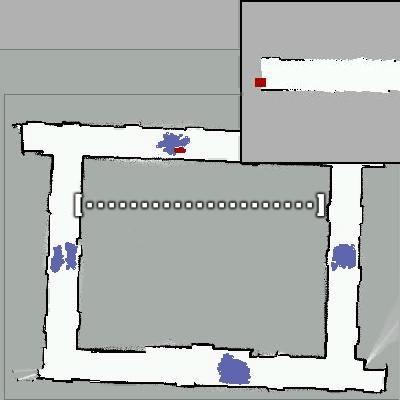
\includegraphics[width=0.6\textwidth]{amcl-still.jpg}}
\end{center}

\foilheadc{VFH+ as a Player driver}
\begin{xitemize}
\item Real-time obstacle avoidance plus local navigation for fast mobile
robots.
\item Supports the standard {\bf position} interface.
\item Works with any laser-equipped robot.
\end{xitemize}
\begin{center}
\begin{tabular}{ccc}
\href{\movieroot/rmp-wallfollow-1.5mps.avi}
{\parbox{0.3\textwidth}
{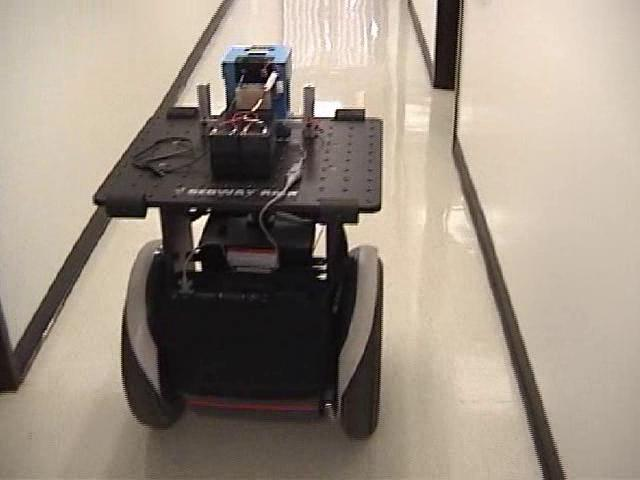
\includegraphics[width=.3\textwidth]{rmp-wallfollow-15mps.jpg}}}
&
\href{\movieroot/rmp-wallfollow-pov.avi}
{\parbox{0.3\textwidth}
{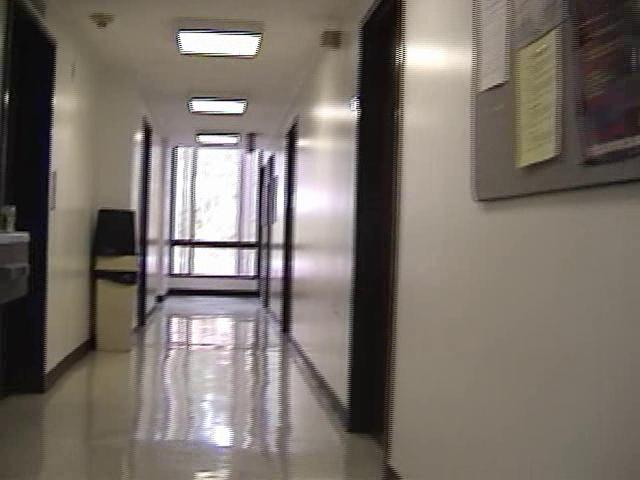
\includegraphics[width=.3\textwidth]{rmp-wallfollow-pov.jpg}}}
&
\href{\movieroot/usc-scilib-day03-clip10.mov}
{\parbox{0.3\textwidth}
{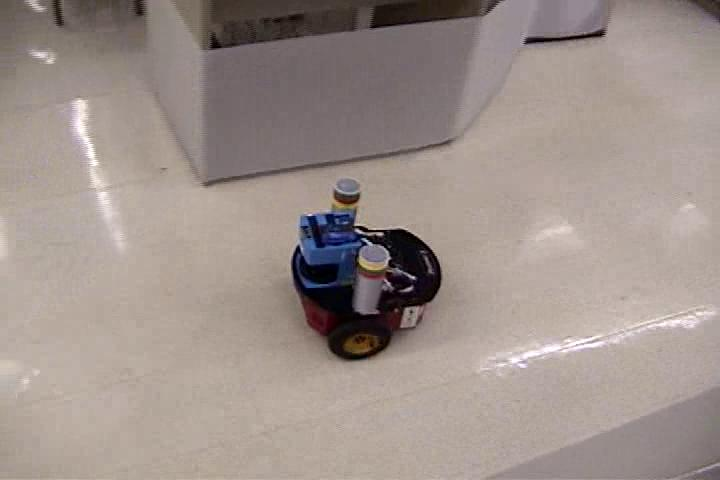
\includegraphics[width=.3\textwidth]{pioneer-vfh.jpg}}}
\end{tabular}
\end{center}

\foilheadc{Resource discovery}
\begin{xitemize}
\item The original Player protocol only provided for access to robot devices
when the full address (host:port:interface:index) is known.
\item Recently added 3 levels of automatic discovery:
{\small
\begin{xitemize}
\item Retrieve the list of available devices from a server.
\item Use the name of a robot to find its port when working in simulation.
\item Full resource discovery across multiple robots on a network, using {\bf
libservicediscovery}, by Reed Hedges @ UMass, Amherst.
\end{xitemize}
}
\end{xitemize}

\foilheadc{Other developments}
\begin{itemize}
\item Support for logging sensor data to files and playing it back as
if live.
\item Utility for producing 2-D maps from laser data.
\item Support for using UDP as transport (almost ready).
\end{itemize}

\foilheadc{Relevance to SDR-II}
{\small
\begin{xitemize}
\item All Player/Stage software is Open Source, released under the GNU
GPL/LGPL.
\item Player runs on many embedded systems (e.g., ipEngine, nanoEngine,
XScale, iPAQ) and on many OSs (e.g., Linux, Solaris, OS~X, FreeBSD).
\item Player supports most research robots, including the AmigoBot and
Pioneer.
\item Player provides much of the underlying functionality necessary for the 
SDR-II task (e.g., localization, mapping, local navigation, fiducial-finding,
acoustic filtering).
\end{xitemize}
}

\foilheadc{Accomplishments}
\begin{itemize}
\item Resource discovery
\item Map-based localization using particle filters
\item Closed-loop control for waypoint-/wall- following
\item Mapping tools
\end{itemize}

\foilheadc{Future work}
\label{lastpage}
\vspace*{-1em}
\begin{xitemize}
\item More closed-loop control in the server, e.g.:
{\small
\begin{xitemize}
\item Impedence controller
\item Target-tracking (visual servoing)
\item Formation-maintenance
\end{xitemize}
}
\item Exploit resource discovery to develop adaptive robot controllers.
\item More high-level capabilities in the server, further making Player a
community code repository, e.g.:
{\small
\begin{xitemize}
\item Path-planning (would enable ``global goto'')
\item Task management (eventually automated allocation)
\end{xitemize}
}
\end{xitemize}

\end{document}
